%%-----------------------------------------------
%
% Include for design chapter of dissertation
%
%%----------------------------------------------

Despite the use of an iterative development methodology, some of the key
components within Partridge were designed 'up front' in order to accelerate
implementation and reduce the time needed to add new components to the
system. The components that make up Partridge and the ways in which they react
are described and analysed below; choices regarding the type of application,
the target audience and the programming environment are also discussed.


\section{ Target Platform \& High Level Considerations }

\subsection{Use Case Analysis}

Given the project objectives identified in \ref{sec:objectives}, four primary
use cases were identified for Partridge as shown in Figure \ref{fig:use_cases}.
Users of Partridge are likely to be researchers who want to find and read
scientific papers. This would involve querying the database for relevant
papers, viewing metrics on the papers that have been used to classify them and
also downloading the original paper for reading. 

Authors are the subset of users who may remain interested in using the query
functionality of Partridge, but also may wish to upload papers to Partridge and
add them to the corpus.

\begin{figure}[!h]
\centering
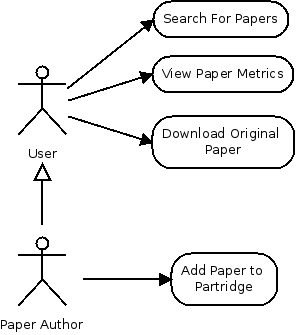
\includegraphics[width=0.4\textwidth]{images/design/use_cases.png}
\caption{Use Case Diagram for Partridge Project}
\label{fig:use_cases}
\end{figure}

\subsection{Target Platform}

From the outset, the aim was that Partridge would be a web-based tool.
Web-based systems can generally be run on any computer with access to the
internet and a modern web browser. This also means that there is no need for
the end user to install or configure extra software on their computers, making
Partridge accessible to non-technical users and those who have aggressive
software restrictions on their computers, such as GPs and the users of public
computers in libraries or on academic sites.

In order to function as a website, Partridge needed to be developed as a server
application that produced Hyper Text Markup Language (HTML) output with which a web
browser could interpret and display. The browser rendering the forms must then
communicate with a backend system capable of querying and returning papers to
the user based on their input. This lead to the decision to split the development
of Partridge into two core components: the Web Frontend comprising of user
interface elements and presentation logic and the Web Backend comprising of
intelligent systems to classify, filter and query papers using some of the NLP
techniques discussed previously.

One of the main requirements for a web server is that it responds to requests
relatively quickly, ideally within 10 seconds or less. If the response is any
slower than this, the user may get impatient and give up trying to use the
system, or in some cases, their web browser may timeout and stop trying to load
the page. Unfortunately, many of the processes involved in extracting meaningful CoreSC
information from papers are very slow. This means that processing papers
during web requests is not really feasible, since it may take several minutes
for a single paper to be annotated and classified. Therefore, a third core
component was identified: a paper preprocessor service that runs on the server
and converts, annotates and classifies papers as soon as they are uploaded.

\subsection{ Programming and Development Environment }

Rather than building a web server from the ground up, most modern web
applications are written in higher level languages that run on top of standard,
open source web servers such as Apache or nginx. Common language choices
include PHP, Python, Perl and Java; all of these languages are supported by large
communities of developers and users who provide with excellent documentation
and support if required.  Python was
selected to implement Partidge. This was partially due to the
author's familiarity with the language and also due to the availability of
stable data mining\cite{curk05} and natural language
processing\cite{bird2009natural} libraries for the Python programming
environment. Python is an interpreted cross-platform language, minimising
deployment problems and supports natively-compiled C and C++ extension
libraries allowing intensive processing  and number crunching to be offloaded
to native plugins, increasing application processing speed.

To further increase development speed, a Python framework for developing web
applications called \emph{Flask} would be used to build the web backend. Flask
is a ``...micro webdevelopment framework for Python.\cite{flask2012}" It
contains a set of utilities and tools for building web applications quickly and
effectively in Python, taking care of low level behaviours such as TCP socket
communication and HTTP requests. These capabilities are presented in a
Model-View-Controller pattern. Flask's capabilities and use within Partridge is
discussed further in Section \ref{sec:backend}.

The development of the application would be carried out on a Linux desktop
computer. However, the portable nature of Python, Apache and the required
libraries meant that Partridge could theoretically be deployed to Windows and
Mac computer systems if required.

The Web Frontend for the system had to be written using a combination of
HTML markup and JavaScript. HTML is not a programming language in itself and
doesn't contain any logic. It is merely a code representation of the interface
to be rendered in the browser window which is interpreted once it has been
downloaded from the web server. In order to carry out actions on the HTML such
as validating user input and manipulating parts of the display, JavaScript is
also downloaded from the web server and interpreted by the browser. Although
this requires the developer to have knowledge of two extra technologies in addition to Python, it also makes enforcing the design principle of keeping presentation
and logic separate a lot easier.

Due to the large number of popular web browsers on the market, implementing
JavaScript in a slightly different way, Javascript can be very difficult to
write in a cross-browser compatible way. To maximise compatibility and reduce
development time, it was decided that jQuery would be used in developing the
JavaScript frontend behaviours. jQuery is a library of utility functions
designed for manipulating HTML documents in a uniform way across all compatible
browsers \cite{jquery2013}. As of February 2013, it is estimated that Chrome and
Firefox are currently the most popular web browsers, holding 50\% and 29.6\% of
the market share respectively\cite{browserstats2013}. Internet Explorer is the
third most popular browser. However, there are several well-known compatibility
issues with Internet Explorer, Microsoft themselves condemning version 6.0\cite{ie6death}. For this reason, it was decided that Partridge
would initially only support Firefox and Chrome; a working interface in modern editions
of the Internet Explorer family of browsers would be a bonus.  However, no time
was allocated to ensuring compatibility of Partridge with Internet Explorer.

\section{ System Architecture }


\begin{figure}[!ht]
\center
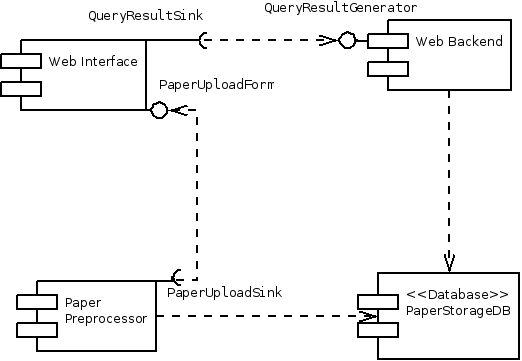
\includegraphics[width=0.6\textwidth]{images/design/components_high_level.png}
\caption{High Level Component Layout for Partridge}
\label{fig:high_level_components}
\end{figure}

Figure \ref{fig:high_level_components} shows a very high level description of
the system's three main components, the database server and the ways that they
communicate. Communication between the Web Interface and the other two
components is carried out via HTTP requests to the underlying Apache server.
Communication between the web backend and the paper preprocessor is implicit
via the data storage system. Direct communication between these components is
redundant since the web backend cannot gain any extra information from the
paper preprocessor while a paper is still being analysed. Furthermore, all finished
papers are added to the database which the web backend has full access to
anyway.


\subsection{ Preprocessor }

The preprocessor module is used to annotate and analyse new papers once they
have been uploaded by the user via the web interface. The preprocessor is
designed as a daemon which hooks into the operating system in order to monitor
a directory for new papers that have been uploaded. As new papers are detected
within the upload directory, they are placed into a process queue and the
preprocessor analyses them on a first in first out basis. When a paper is taken
from the queue, a series of processes are run upon it to prepare it for storage
in the database. These processes are illustrated in Figure
\ref{fig:flow_preprocessor}.

\begin{figure}[!h]
\centering
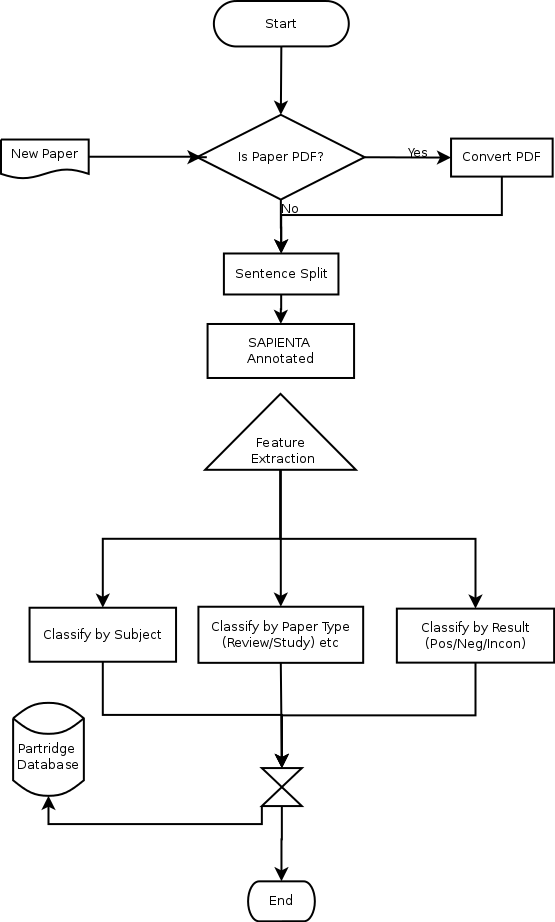
\includegraphics[width=0.6\textwidth]{images/design/flow_preprocessor.png}
\caption{A flowchart illustrating the preprocessor processes}
\label{fig:flow_preprocessor}
\end{figure}

\subsubsection{PDF to XML Conversion}

The first process in the processing pipeline is conversion of the papers to a
format that can be analysed by SAPIENTA. Currently, SAPIENTA supports the
SciXML\cite{rupp2006flexible} and PubMed Central\cite{pubmedDTD} DTDs. However,
papers stored in PDF format must still be converted in order to be processed.
PDF Files will passed through a routine which extracts text from the paper and
adds the relevant XML tags to make the document SAPIENTA compatible. This
document is then passed forward to the splitter. Papers that are already in a
compatible format are passed forward without any action being taken.

\subsubsection{Sentence Splitting} 

SAPIENTA allocates each sentence within a paper a separate CoreSC label.
However, the sentence boundaries must be detected before the document is passed
into SAPIENTA for annotation. The sentence splitter uses a regular expression
to split the sentences within the document and then adds the necessary
\verb|<s>| tags to the markup to indicate the location of each sentence.

\subsubsection{SAPIENTA Annotation}

Once the paper has been split, SAPIENTA is used to annotate each sentence with
a relevant CoreSC label. These labels are calculated based upon the
sentence's location within the paper as well pairs and triplets of words found
consecutively within the sentence. After this stage, the paper is passed
forwards to be further classified by Partridge.


\subsubsection{Feature Extraction and Classifiers}

The final stage in the preprocessor pipeline is paper classification. During
this stage, features wil be extracted from the papers and used to classify the
paper in three different ways. The paper's type: case study or review paper
etc. will be determined using the presence or absence of different CoreSC labels
within the paper and their relative proportions. The subject of paper will be
determined by the presence of domain specific nouns and adjectives within the
paper. For example, a biology paper might contain words such as 'enzyme' or 'amino
acid.' The result of the paper, i.e. whether the paper was conclusive and if the
results were positive or negative, will be detected through the presence or absence
of words with a strong sentiment polarity as discussed by Wilson et al
(2005)\cite{Wilson05Polarity}. The results from the whole process are then
passed into the data store and saved.

\subsubsection{File Retention and Error Handling}

Each of the independent processes described above generate new files which are
temporarily stored on the server until all of the sub-processes are complete.
Once a paper analysis cycle has finished, the preprocessor triggers a cleanup
operation that removes intermediate files from the system, storing only the
initially uploaded file (which may be a PDF) and the final annotated file in a
permanent location on the filesystem.  The whole analysis process for a single
paper is also wrapped within an error handling block that automatically
executes the cleanup routine if something goes wrong. This prevents the system
filling up with invalid files. This mechanism is shown in Figure
\ref{fig:preprocessor_overview}.

\begin{figure}[!h]
\vspace{5mm}
\centering
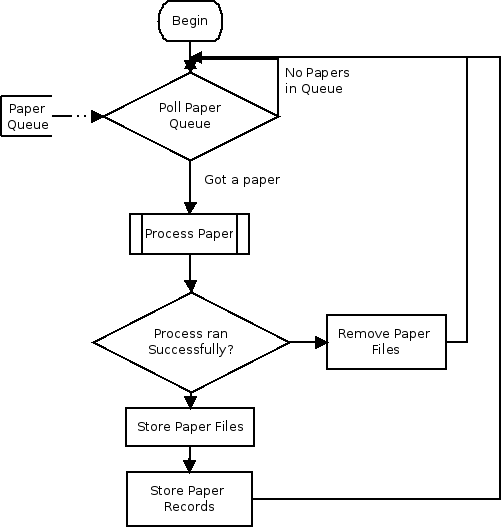
\includegraphics[width=0.6\textwidth]{images/design/paper_processor_overview.png}
\caption{Preprocessor System Overview}
\label{fig:preprocessor_overview}
\end{figure}


\subsection{ Data Storage }
\label{sec:db_layout}
It is expected that Partridge may grow in size to contain
tens of thousands of individual papers that have been annotated and are available to
the web backend for inclusion into a user's search results. Reading and
parsing each individual XML file stored in the system is not really feasible
when handling a HTTP request from the web frontend, this sort of process would
take a long time to execute. To provide fast search and retrieval of paper
data, a Relational Database Management server (RDBMS) was chosen for storage of
papers that have been preprocessed using the system described above. An
overview of the database schema is illustrated in Figure \ref{fig:e-r-diagram}.

\begin{figure}[th]
\vspace{5mm}
\centering
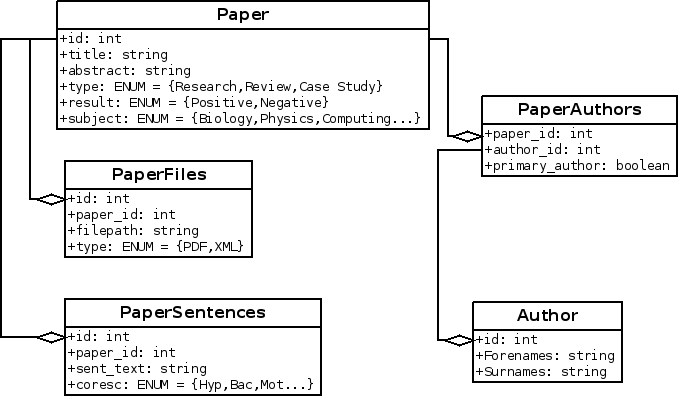
\includegraphics[width=0.8\textwidth]{images/design/e-r-diagram.png}
\caption{Entity Relationship Diagram for Partridge's RDBMS}
\label{fig:e-r-diagram}
\end{figure}

Partridge's database is required to keep track of all of the papers that have
been added to the system. The Paper entity represents a single paper stored in
Partridge. Information is extracted and classified by indicators such as the paper's type,
topic and resul. This is are stored as part of the main paper entity. The title and
topic are also stored for easy retrieval. One of the key requirements of
Partridge is querying within a CoreSC field of a paper. Therefore, all
sentences are stored as entities along with their CoreSC annotation. The sentence
text is an index field to facilitate fast recall from the database.

It is probable that any given author may have contributed to multiple papers
stored within the system.  Therefore authors are treated as entities within the
RDBMS and the many to many relationship between papers and authors is
facilitated using the intermediary table PaperAuthors. A PaperAuthor record
contains a boolean field used to indicate whether the author that is linked to a
specific paper was the primary author on that paper.

As discussed above, two or more files per paper are always stored within
Partridge so that a user can retrieve them for reading. Therefore files are
kept in their own table along with a record of their type (eg. XML or PDF). 

\subsection{ Web Backend }

Partridge's web backend component is used to initially serve the HTML and
JavaScript used to represent the User interface and to communicate with the
JavaScript frontend running inside the browser via HTTP requests. It is used to
interpret HTTP request fields into SQL queries and mediate queries made to the
RDBMS on behalf of the user. An example use of the backend system can be seen
in Figure \ref{fig:backend_sequence}.

\begin{figure}[!ht]
\centering
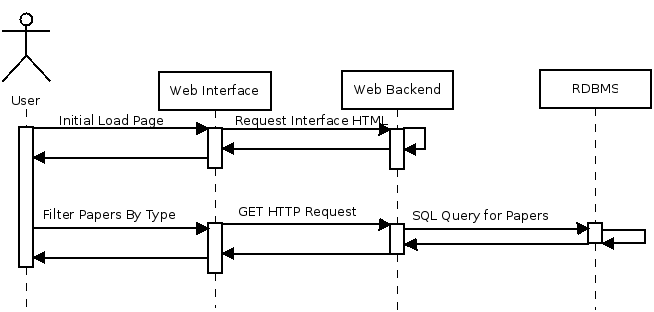
\includegraphics[width=0.75\textwidth]{images/design/backend_sequence.png}
\caption{Sequence Diagram for a Query in Partridge}
\label{fig:backend_sequence}
\end{figure}

The Flask web framework uses a model view controller-like architecture. Each
behaviour of the server, handling paper uploads, displaying paper query
results and allowing users to download papers, can be considered a `view'. Views
register themselves with Flask under a specific URL. When Flask receives a
request to any such URL, it automatically routes the request through to the
View object\cite{flask2012}.

\subsubsection{Query View Backend}
The query view is has two key responsibilities. The first is to display the
query form to the user. This is a simple matter of sending an HTML file stored
on the server to the browser that made the request. 

The key responsibility of the query view is to translate incoming HTTP requests
into search queries, retrieve a set of papers from the RDBMS  and return human
readable results to the user. One of the most important steps in this process
is to cleanse the incoming data and prevent SQL injection attacks that
unscrupulous users may attempt to use to damage or purge the Partridge
database. These are handled transparently by the SQLAlchemy library as
discussed in Section \ref{sec:dbandsqlalchemy}. The system must also be capable
of interpreting data retrieved from the database into HTML to be returned to
the user's browser. The server mechanism utilises Flask's built in templating
mechanism in order to quickly transform Python-specific data structures into
valid HTML markup and return it to the user\cite{flask2012}.

\subsubsection{Paper Upload View Backend}

The paper upload view backend is responsible for handling file uploads from the
HTML form and ensuring that files are placed in the right place so that the
preprocessor can find them. The main challenge for this submodule is storing
the file using a unique name so that different users uploading files don't
overwrite each other's data. This is handled through the use of the Python UUID
module which generates universally unique 128-bit identifiers as detailed in RFC
4122\cite{rfc4122}. The low rate of collisions between UUID values should
insure that the chances of two paper filenames colliding is very low. 

The view also carries out validation on the filename to ensure that it is an
XML or PDF file. No further validation is carried out by this system since the
paper processor carries out file contents inspection and removes invalid file
types automatically.


\subsection{ Web Frontend }
\label{sec:web_frontend}

The web frontend consists of sets of HTML and JavaScript interfaces that are
equipped to communicate with the backend systems discussed above using HTTP
requests. The most important aspect in designing the frontend was insuring that
the interfaces are intuitive and usable from the perspective of a non-technical
user. It was suggested that the system should look as similar as possible to
other online search and information retrieval systems in order to help users
who are already familiar with other systems in learning to use Partridge more
quickly.

\subsubsection{ Query Form }

\begin{figure}[!htb]
\vspace{5mm}
\centering
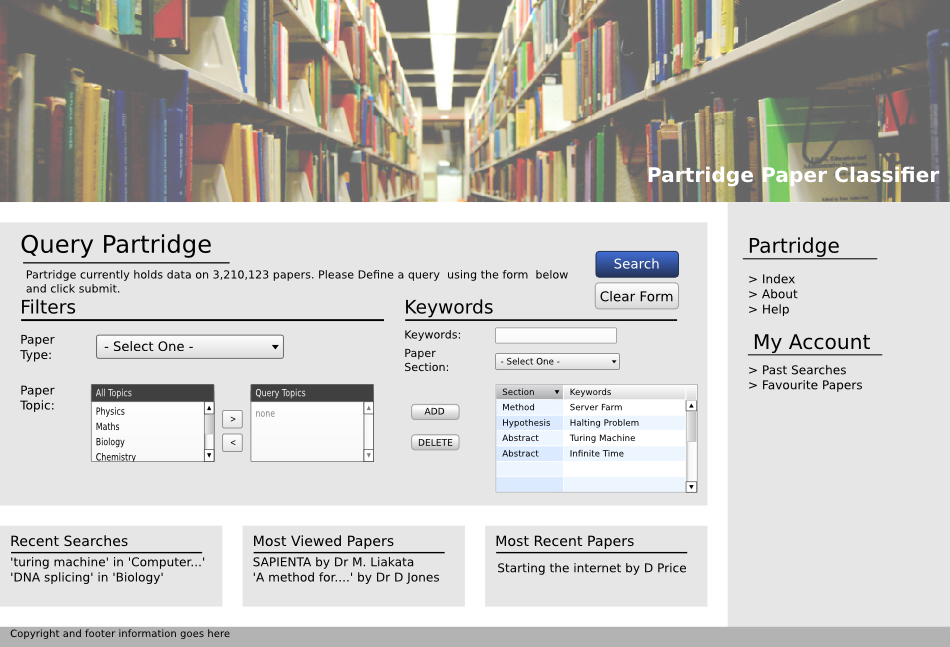
\includegraphics[width=\textwidth]{images/design/query_mockup.png}
\caption{Mockup image for the Partridge Query Interface}
\label{fig:query_mockup}
\end{figure}

Figure \ref{fig:query_mockup} shows the initial design of the Partridge query
interface. The interface tries to make it easy for the user to both filter and
query papers in an intuitive way.

The filter interface on the left hand side of the query form allows the user to
use Partridge's machine learning classifiers to return subsets of the papers.
The selection box control in the top left of the form contains a list of each
of the types of paper within the database. The user should select one of these
types of paper to restrict their query to that type. There is also an ``All
Types" option in case they don't wish to use this filter.

The paper topic filtering system is displayed in the bottom left of the query
form. There is a `master list' of all paper topics in the corpus on the left
and a `query list' containing topics that the user wants to be included into
their search results on the right. The user selects items from each list and
can use the arrow buttons in between to move them depending on their query.

The search or `Keywords' section of the form shows a set of controls for
specifying terms that must appear within sections of a document in order to show
up in the search results. The user enters a search term in the input box on the
top right of the form and then selects which section of the paper the term
should appear within. This could be any of the CoreSC labels within the paper or
within the abstract. The user could also specify a specific author's name. Once
they are happy with their keywords and section, they click `Add' and the
keyword/section pair are inserted into the table on the bottom right. If they
wish to remove a query constraint from this table, they can select it and click
the `Delete' button. 

Once the user is happy with their search, they can click the `Search' button
at the extreme top right of the form to carry out the query and see the
results.

\subsubsection{ Results Page }

After the user has made their query, the results are displayed for them
to find relevant papers to read. Figure \ref{fig:results_mockup} shows a
mockup of the results view. This page clearly lists all of the papers found
during the query in order of relevence. The results are paginated so that the user
does not have to wait for a large page to render. It is hoped that users will
run such specific queries that they do not return a high number of results. There is a
prominent link at the top of the page that allows the user to go back to the
query form and amend their query if the results are not satisfactory.

\begin{figure}[!htb]
\vspace{5mm}
\centering
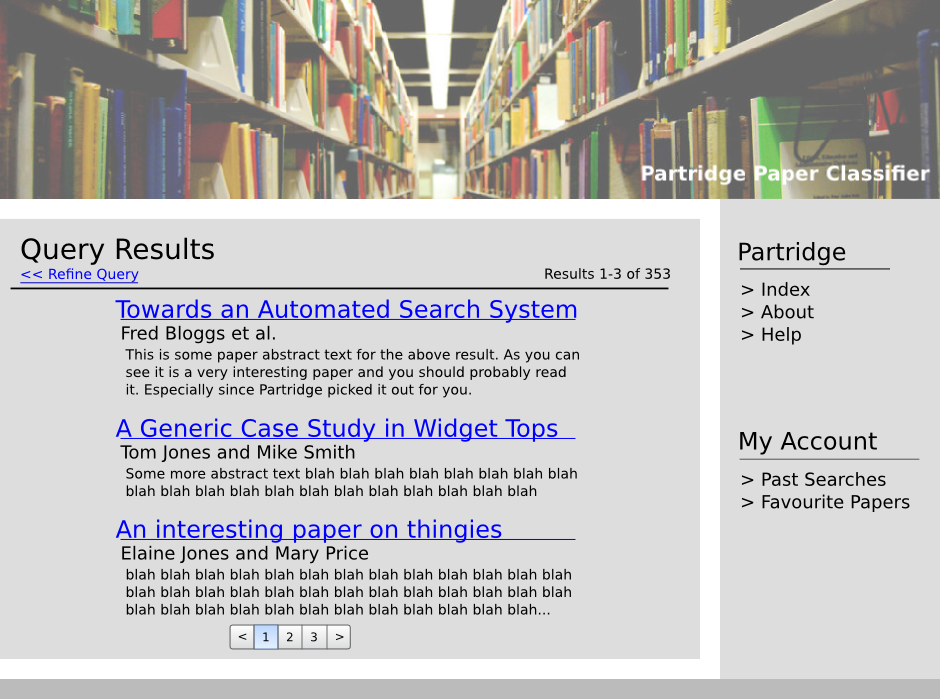
\includegraphics[width=\textwidth]{images/design/results_mockup.png}
\caption{Mockup image for the Partridge Search Results Interface}
\label{fig:results_mockup}
\end{figure}

Each paper is listed by title and author and the first few sentences of the
extract are also dislayed. The user can click on the paper title to be taken to
the Profile Page for that paper.


\subsubsection{ Paper Profile Page }

The paper profile page is used to display all information about a specific
paper in the Partridge corpus to the user. A mockup of the Paper Profile page
can be seen in Figure \ref{fig:paper_profile}

\begin{figure}[!htb]
\vspace{5mm}
\centering
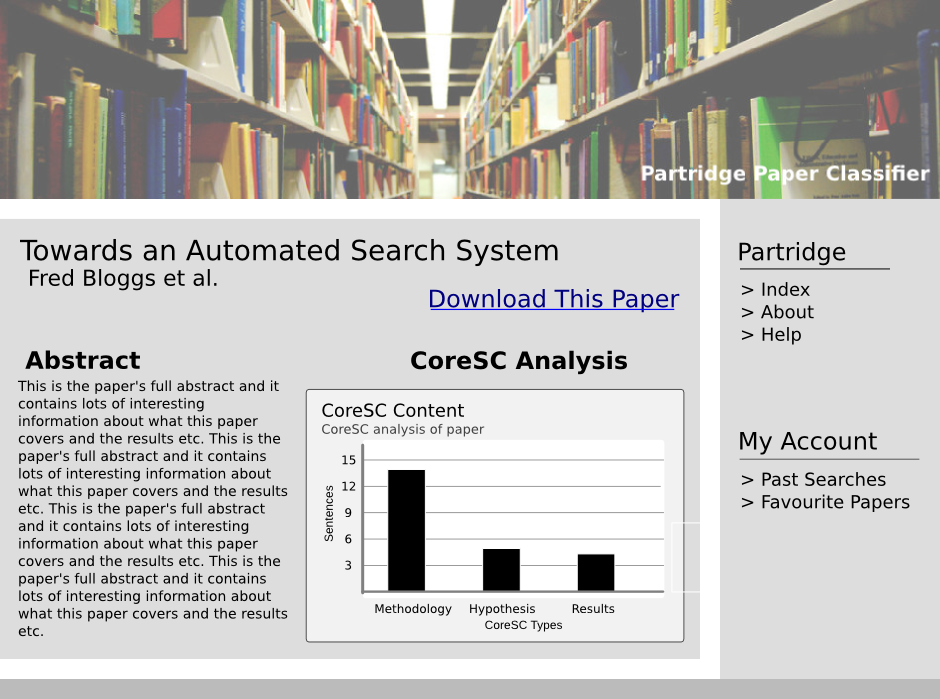
\includegraphics[width=\textwidth]{images/design/profile_mockup.png}
\caption{Mockup image for the Partridge Paper Profile Page}
\label{fig:paper_profile}
\end{figure}

The paper's title and author are displayed prominently in the top left hand
corner of the page. The full text of the abstract is shown so that the user can determine the paper's relevance to them. There is also a graph showing
each of the CoreSC types and proportion within the paper (the example chart only
shows three CoreSC label types for brevity). If the user is
interested in the paper, they can click the Download link at the top of the
page to access the annotated XML file stored in the system.

\subsubsection{Paper Upload Form}
Paper uploading is another very important user activity within Partridge.
Without users uploading papers, Partridge has no data to work with. It was
therefore, very important to make paper uploading as easy as possible to
the end user. Figure \ref{fig:paper_upload} shows Partridge's main paper upload
form. 

\begin{figure}[!htb]
\vspace{5mm}
\centering
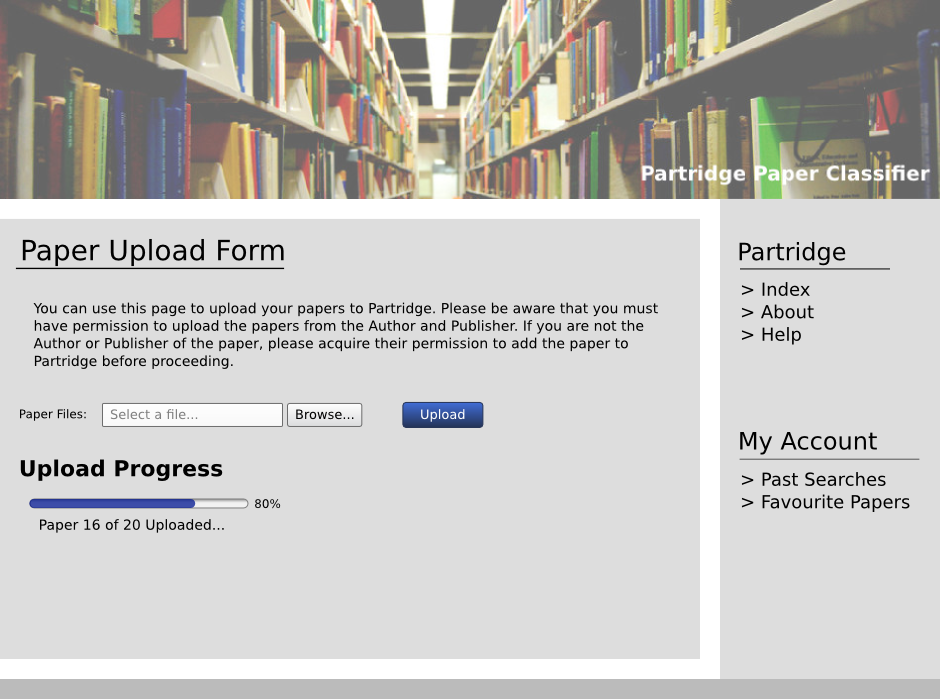
\includegraphics[width=\textwidth]{images/design/upload_mockup.png}
\caption{Mockup image for the Partridge Paper Upload Form}
\label{fig:paper_upload}
\end{figure}

The papers are selected using the familiar File Upload dialog used in any
website that requires users to upload files to the server. Multiple papers can
be selected for batch upload if required. Once the relevant papers are
selected, the user selects the Upload button to begin the process. 

Once the upload process has started, the upload file browser and submit button
are disabled and a progress indicator as well as a text summary are displayed
directly underneath. Once the progress bar reaches 100\%, the upload file
browser becomes available again, or the user can navigate away from the page.

\section{ Summary}

All of Partridge's subsystems have carefully been designed in order to make
programming and implementing the project efficient and easy for the programmer.
The system architecture allows the implementation of modules independantly of
each other with minimal coupling and communication. Cohesion within the modules
is maximised, with related behaviours grouped together as far as possible.

The user interface has been designed to maximise usability for non-technical
users whilst effectively encoding the complicated nature of Partridge's
internal processes in a set of HTML forms.

Partridge has been developed using an iterative methodology and therefore some
of the designs discussed in this chapter have been modified during the
development of the project. However, these designs did provide an excellent
starting point for the implementation of the project.
